\documentclass[10pt]{beamer}
\usepackage{graphicx}
\usepackage{cancel}
\usepackage{bbold}
%\usepackage{caption}

\usetheme{Szeged}
\usecolortheme{dolphin}
%\definecolor{unitn-gray}{HTML}{b4aba2}
%\definecolor{unitn-blue}{HTML}{01448a}

\title{Bell's theorem without inequalities}
%\author{Severino Zeni}
\institute{Severino Zeni}%to have my name instead of unitn on slides
\date{September 26, 2014}

\begin{document}
%  \frame{\titlepage}

\begin{frame}
  \thispagestyle{empty}
  \begin{center}
    
\includegraphics[width=4.5cm]{Images/logo-unitn.jpg}\\[-0.1cm]
    {\small Department of Physics}\\[0.6cm]
    {\small Degree in Physics}\\[0cm]
    {\small Thesis}\\[-0.1cm]
    % Title
    \rule{\linewidth}{0.2mm}\\[0.3cm]
    { \Large \bfseries Bell's theorem without inequalities}\\[0cm]
    \rule{\linewidth}{0.2mm}\\[0.5cm]
    % Author and supervisor
    \begin{minipage}{0.4\textwidth}
      \begin{flushleft} \small
        \emph{Supervisor:} \\[0cm]
        Prof. Franco Dalfovo
      \end{flushleft}
    \end{minipage}
    \begin{minipage}{0.4\textwidth}
      \begin{flushright} \small
        \emph{Student:}\\[0cm]
        Severino Zeni
      \end{flushright}
    \end{minipage}\\[0.6cm]
    \vfill
    {\small September 26, 2014}
  \end{center}
\end{frame}




\begin{frame}
  \frametitle{Table of contents}
  \tableofcontents
\end{frame}

\section{EPR and Bell's results}
\subsection{The EPR ``theorem''}
\begin{frame}{Perfect correlations in systems of two spin-1/2 particles}
  For systems of two spin-1/2 particles in the state (singlet state):
  \begin{equation*}
    |\chi\rangle = \frac{1}{\sqrt{2}} \left( |+\rangle_1 |-\rangle_2 - |-\rangle_1 |+\rangle_2 \right)
    \label{eq:singlet-state}
  \end{equation*}
  QM predicts opposite results if the same spin component is measured on both particles.
\end{frame}




\begin{frame}{EPR argument}
  \begin{columns}[c] % the "c" option specifies center vertical alignment
    \column{.51\textwidth} % column designated by a command
    \begin{figure}
      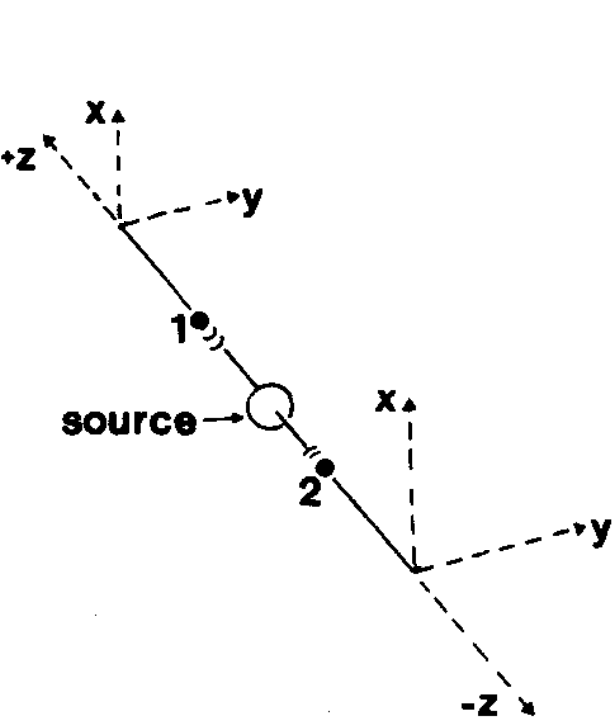
\includegraphics[width=3.5cm]{Images/eprb-gedankenexperiment.png}
      \caption{The Bohm gedankenexperiment. Credits \cite{:/content/aapt/journal/ajp/58/12/10.1119/1.16243}.}
      \label{fig:eprb-gedankenexperiment}
    \end{figure}
    \column{.55\textwidth}
    \begin{itemize}
    \item \textbf{Perfect correlation:} see previous slide.
    \item \textbf{Locality:} if the two particles are far from each other, measurements on one particle do not change the elements of physical reality of the other particle.
    \item \textbf{Reality:} If the result of a measurement can be predicted with certainty, there exists an element of physical reality corresponding to the measured quantity.
    \end{itemize}
    \begin{center}
      {\Large $\Downarrow$}\\[0.1cm]
      \textbf{QM is incomplete}
    \end{center}
  \end{columns}
\end{frame}




\subsection{Summary of Bell's contribution}
\begin{frame}{Bell's formalization of EPR's results}
  Let $\lambda$ be the complete description of pairs in the singlet state, then:
  \begin{equation*}
    \text{Results of measurements on particle 1} ~~ \longrightarrow ~~ A = A_{\mathbf{\hat{u}}}(\lambda)
  \end{equation*}
  \begin{equation*}
    \text{Results of measurements on particle 2} ~~ \longrightarrow ~~ B = B_{\mathbf{\hat{v}}}(\lambda)
  \end{equation*}
where ${\mathbf{\hat{u}}}$ and ${\mathbf{\hat{v}}}$ indicate the spin component measured.\\[1cm]
Because of locality $A$ depends on ${\mathbf{\hat{u}}}$ and not on ${\mathbf{\hat{v}}}$, $B$ depends on ${\mathbf{\hat{v}}}$ and not on ${\mathbf{\hat{u}}}$.
\end{frame}




\begin{frame}{Bell's inequality}
Let $E(\mathbf{\hat{u}}, \mathbf{\hat{v}})$ be the expectation value of the product of the two particles' spin components. Using the objects just introduced:
\begin{equation*}
  E(\mathbf{\hat{u}}, \mathbf{\hat{v}}) = \int \rho(\lambda) A_{\mathbf{\hat{u}}}(\lambda) B_{\mathbf{\hat{v}}}(\lambda) d\lambda
\end{equation*}
where $\rho(\lambda)$ is the probability distribution of the $\lambda$'s.




Then Bell proved that, for any theory that obeys the EPR assumptions:
\begin{equation*}
  \left| E(\mathbf{\hat{u}}, \mathbf{\hat{v}}) - E(\mathbf{\hat{u}}, \mathbf{\hat{w}}) \right| - E(\mathbf{\hat{v}}, \mathbf{\hat{w}}) \leq 1
  \label{eq:bell-inequality}
\end{equation*}

But for $\mathbf{\hat{u}}$, $\mathbf{\hat{v}}$ and $\mathbf{\hat{w}}$ in the $xy$ plane with azimuthal angles $0^\circ$, $60^\circ$ and $120^\circ$ respectively, QM predicts:
\begin{equation*}
  \left| E(\mathbf{\hat{u}}, \mathbf{\hat{v}}) - E(\mathbf{\hat{u}}, \mathbf{\hat{w}}) \right| - E(\mathbf{\hat{v}}, \mathbf{\hat{w}}) = \frac{3}{2},
\end{equation*}
Thus, \emph{statistical predictions} of QM contradict EPR's assumptions.
\end{frame}




\section{GHZ theorem}
\subsection{Adaptation to systems of three spin-1/2 particles}
\begin{frame}{Perfect correlations in systems of three spin-1/2 particles}
Consider a system of three spin-1/2 particles in the state:
\begin{equation*}
  |\chi\rangle = \frac{1}{\sqrt{2}} \left( |+\rangle_1 |+\rangle_2 |+\rangle_3 - |-\rangle_1 |-\rangle_2 |-\rangle_3 \right)
  \label{eq:ghz-state}
\end{equation*}
where $|+\rangle_i$ and $|-\rangle_i$ are taken along the $\mathbf{\hat{z}}$ direction.

If we measure a spin component of each particle, in particular the triples of observables:
\begin{equation*}
  \begin{split}
    \left( S_{1x} \times \mathbb{1}_2 \times \mathbb{1}_3,~~~ \mathbb{1}_1 \times S_{2y} \times \mathbb{1}_3,~~~ \mathbb{1}_1 \times \mathbb{1}_2 \times S_{3y} \right)\\
    \left( S_{1y} \times \mathbb{1}_2 \times \mathbb{1}_3,~~~ \mathbb{1}_1 \times S_{2x} \times \mathbb{1}_3,~~~ \mathbb{1}_1 \times \mathbb{1}_2 \times S_{3y} \right)\\
    \left( S_{1y} \times \mathbb{1}_2 \times \mathbb{1}_3,~~~ \mathbb{1}_1 \times S_{2y} \times \mathbb{1}_3,~~~ \mathbb{1}_1 \times \mathbb{1}_2 \times S_{3x} \right)
  \end{split}
  \label{eq:xyy-observables-triplets}
\end{equation*}
QM predicts that the result of the measurement of any observable in a triple is completely determined once the other two observables in the triple are measured.
\end{frame}




\begin{frame}{EPR premises adapted to three particles}
  The EPR premises hold also in the case of three particles:
  \begin{itemize}
  \item \textbf{Perfect correlation:} see previous slide.
  \item \textbf{Locality:} if the particles are far from each other, measurements on one particle do not change the elements of physical reality of the other particles.
  \item \textbf{Reality:} If the result of a measurement can be predicted with certainty, there exists an element of physical reality corresponding to the measured quantity.
  \end{itemize}
  \begin{center}
    {\Large $\Downarrow$}\\[0.2cm]
    There exists a more complete state specification $\lambda$;\\
    Results of spin component measurements are given by:
    \begin{equation*}
      A = A_i(\lambda),~ B = B_j(\lambda),~ C = C_k(\lambda)
    \end{equation*}
    for particle 1, 2 and 3 respectively.% ($i, j, k = x, y$)
  \end{center}
\end{frame}




\subsection{GHZ theorem}
\begin{frame}{GHZ argument}
  QM predicts for the product of three spin components (on the state of two slides ago):
  \begin{equation*}
    \begin{matrix}
      \mathcal{P}(S_{1x} \times S_{2y} \times S_{3y} = 1) = 1 & \Rightarrow & A_x B_y C_y = 1\\
      \mathcal{P}(S_{1y} \times S_{2x} \times S_{3y} = 1) = 1 & \Rightarrow & A_y B_x C_y = 1\\
      \mathcal{P}(S_{1y} \times S_{2y} \times S_{3x} = 1) = 1 & \Rightarrow & A_y B_y C_x = 1\\[.2cm]
      & & \text{{\large $\Downarrow$}}\\[.2cm]
      & & A_x B_x C_x = 1
    \end{matrix}
  \end{equation*}
  But QM also predicts:
  \begin{equation*}
      \mathcal{P}(S_{1x} \times S_{2x} \times S_{3x} = - 1) = 1 ~~ \Rightarrow ~~ A_x B_x C_x = - 1
  \end{equation*}
  Thus \emph{certain predictions} of QM contradict EPR's assumptions.
\end{frame}




\begin{frame}{Statement of the GHZ theorem}
  \begin{theorem}
    One (at least) of the following statements is false:
    \begin{itemize}
    \item Nature is compatible with the \textbf{locality} assumption.
    \item Nature is compatible with the \textbf{reality} assumption.
    \item QM gives correct predictions for \textbf{perfect correlations}.
    \end{itemize}
  \end{theorem}
\end{frame}




\section{Experimental observations}
\subsection{Ideal experiment}
\begin{frame}{Ideal experiment}
  The state $\frac{1}{\sqrt{2}} \left( |+\rangle_1 |+\rangle_2 |+\rangle_3 - |-\rangle_1 |-\rangle_2 |-\rangle_3 \right)$ is an eigenstate of all the observables considered:
  \begin{equation*}
    \begin{split}
      &S_{1x} \times S_{2y} \times S_{3y}\\
      &S_{1y} \times S_{2x} \times S_{3y}\\
      &S_{1y} \times S_{2y} \times S_{3x}\\
      &S_{1x} \times S_{2x} \times S_{3x}.
    \end{split}
  \end{equation*}
  Moreover, all these observables commute with each other.\\[.5cm]
  Thus, it is possible to measure all four products at the same time, i.e. a single run (with a single triplet) of the experiment suffices to confirm or disprove QM against local-realism.\\[.2cm]
  To our knowledge no experiment of this type has been performed.
\end{frame}




\subsection{Observation of GHZ entanglement}
\begin{frame}{Interferometer}
  \begin{columns}[c]
    \column{.5\textwidth}
    \begin{figure}
      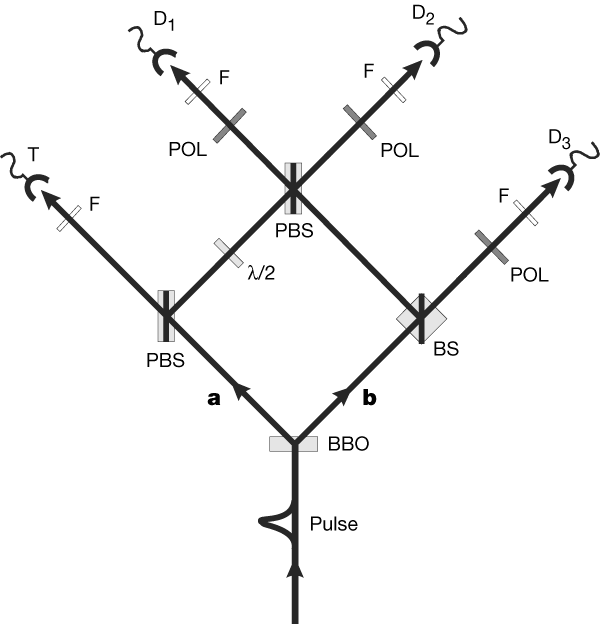
\includegraphics[width=0.9\textwidth]{Images/ghz-entanglement'.png}
      \caption{Schematic drawing of the interferometer. Credits \cite{Nature.403.515}.}
    \end{figure}
    \column{.5\textwidth}
    UV pulses generate pairs of photons in (polarization) state:
    \begin{equation*}
      \frac{1}{\sqrt{2}} \left( |H\rangle_a |V\rangle_b - |V\rangle_a |H\rangle_b \right).
    \end{equation*}
    If two pairs are generated by a single UV pulse and all four detectors fire, then at $D_1$, $D_2$ and $D_3$ we observe either of the following states:
    \begin{equation*}
      \begin{split}
        &|H\rangle_1 |H\rangle_2 |V\rangle_3\\
        &|V\rangle_1 |V\rangle_2 |H\rangle_3
      \end{split}
    \end{equation*}
    An intensity ratio of $12:1$ is observed between the desired and undesired states.
  \end{columns}
\end{frame}




\begin{frame}{Condition for coherent superposition}
  The couple of pairs is generated in the state:
  \begin{equation}
    \frac{1}{2} \left( |H\rangle_a |V\rangle_b - |V\rangle_a |H\rangle_b \right) \left( |H\rangle'_a |V\rangle'_b - |V\rangle'_a |H\rangle'_b \right).
    \label{eq:double-dc-state}
  \end{equation}
  Single component's evolution in the interferometer is given by:
  \begin{center}
    \renewcommand{\arraystretch}{1.5}
    \begin{tabular}{l r}
      $|H\rangle_a \rightarrow |H\rangle_T$ & $|V\rangle_a \rightarrow \frac{1}{\sqrt{2}} \left( |V\rangle_1 + |H\rangle_2 \right)$\\
      $|V\rangle_b \rightarrow \frac{1}{\sqrt{2}} \left( |V\rangle_2 + |V\rangle_3 \right)$ & $|H\rangle_b \rightarrow \frac{1}{\sqrt{2}} \left( |H\rangle_1 + |H\rangle_3 \right)$
    \end{tabular}\\
    \end{center}
  Substituting these into (\ref{eq:double-dc-state}) and dropping unwanted terms leads to:
  \begin{equation*}
%    \frac{1}{2} \left(
|H\rangle_T \left( |H\rangle'_1 |H\rangle'_2 |V\rangle_3 + |V\rangle'_1 |V\rangle_2 |H\rangle'_3 \right) + |H\rangle'_T \left( |H\rangle_1 |H\rangle_2 |V\rangle'_3 + |V\rangle_1 |V\rangle'_2 |H\rangle_3 \right)
% \right)
  \end{equation*}
  Finally, if unprimed and primed photons are indistinguishable:
  \begin{equation*}
    \frac{1}{\sqrt{2}} |H\rangle_T \left( |H\rangle_1 |H\rangle_2 |V\rangle_3 + |V\rangle_1 |V\rangle_2 |H\rangle_3 \right).
  \end{equation*}
\end{frame}




\begin{frame}{How to render the photons indistinguishable?}
  \begin{columns}[c]
    \column{.5\textwidth}
    \begin{figure}
      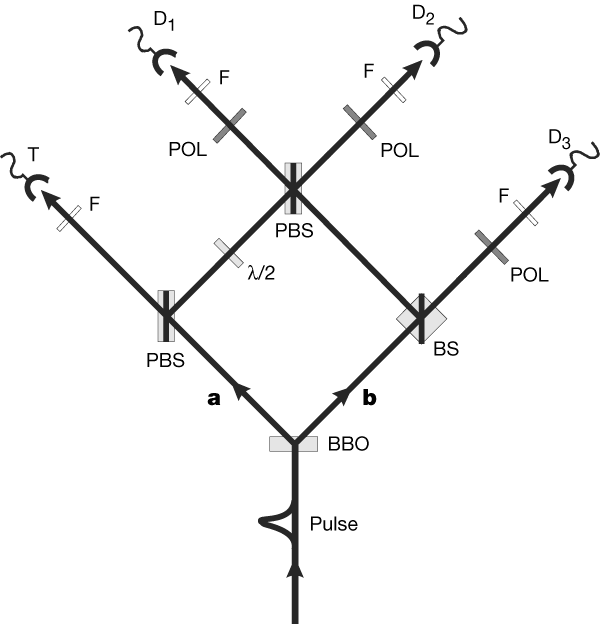
\includegraphics[width=0.9\textwidth]{Images/ghz-entanglement'.png}
      \caption{Credits \cite{Nature.403.515}.}
    \end{figure}
    \column{.5\textwidth}
    Primed and unprimed photons can be distinguished by:
    \begin{itemize}
    \item Energy conservation.
    \item Timing of detection.
    \end{itemize}
    The use of narrow interference filters in front of the detectors cancels the possibility of distinguishing the photons.
  \end{columns}
\end{frame}




\begin{frame}{Method to experimentally confirm GHZ entanglement}
  A measurement of $+45^\circ$ polarization on photon 1 projects the coherent state into:
  \begin{equation*}
    \frac{1}{\sqrt{2}} |H\rangle_T |+ 45^\circ\rangle_1 \left( |H\rangle_2 |V\rangle_3 + |V\rangle_2 |H\rangle_3 \right),
  \end{equation*}
  that written on the $( |+ 45^\circ\rangle_i, |- 45^\circ\rangle)_i$ bases, for photon 2 and 3 gives:
  \begin{equation*}
    \begin{split}
      \frac{1}{2 \sqrt{2}} \left( |+\rangle_2 |+\rangle_3 - \cancel{|+\rangle_2 |-\rangle_3} + \cancel{|-\rangle_2 |+\rangle_3} - |-\rangle_2 |-\rangle_3 + \right.\\
      \left. + |+\rangle_2 |+\rangle_3 + \cancel{|+\rangle_2 |-\rangle_3} - \cancel{|-\rangle_2 |+\rangle_3} - |-\rangle_2 |-\rangle_3 \right).
    \end{split}
  \end{equation*}
  The terms $|+\rangle_2 |-\rangle_3$ and $|-\rangle_2 |+\rangle_3$ interfere destructively. Hence, the observation of the terms $|+\rangle_2 |+\rangle_3$ and $|-\rangle_2 |-\rangle_3$ is a proof of coherence.
\end{frame}





\begin{frame}{Experimental confirmation of GHZ entanglement}
  \begin{figure}
    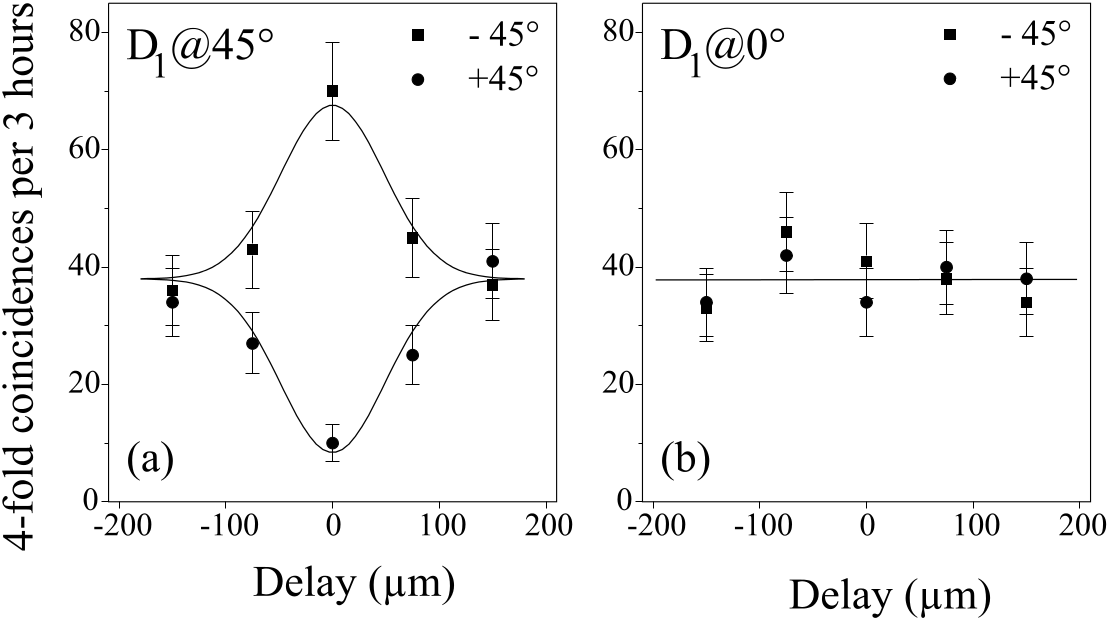
\includegraphics[width=0.6\textwidth]{Images/ghz-entanglement-exp-proof.png}
    \caption{Results for polarization analysis of photon 3, conditioned on the detection of photon 1 polarized at $+ 45^\circ$ and photon 2 polarized at $- 45^\circ$. The (spatial) delay refers to a change in path $a$ introduced to show that coherence is lost if photons can be distinguished. By comparison (graph (b)) no intensity difference is predicted if the polarizer in front of the detector $D_1$ is set at $0^\circ$. Credits \cite{PhysRevLett.82.1345}.}
  \end{figure}
%  \begin{columns}
%    \column{.5\textwidth}
%    \coulmn{.5\textwidth}
%  \end{columns}
\end{frame}

\section*{}
\begin{frame}{Conclusion - Claims regarding local realism}
  The experimental procedure and analysis presented doesn't allow claims in favor or against QM to be made.\\[1cm]% That is because...ADD EXAMPLE OF SOME REASON\\[1cm]
  However, such claims are present in the literature. It has been shown that a more refined analysis of the data, coming from an improved version of the interferometer presented, allows to make claims against local-realism.\\
However, the analysis of these claims is beyond the scope of this thesis.
\end{frame}

\begin{frame}{Conclusion - By-product}
  The study of the matter with which this thesis is concerned allowed us to observe:
  \begin{itemize}
%  \item To the same self-adjoint operator there may correspond different experimental apparatuses that perform different projections.
  \item Entanglement does not necessarily arise from interaction of the entangled systems.
  \end{itemize}
\end{frame}



\begin{frame}
  \frametitle{Summary}
  \tableofcontents
\end{frame}



\begin{frame}
  \frametitle{Bibliography}
  \bibliography{bibliography}
  \bibliographystyle{unsrt}
\end{frame}

\end{document}
